% Provenance (never printed): old seconde/premiere S material on soil as a
% slowly renewed resource (alteration of rocks, clays, the clay--humus
% complex, soil erosion); see sources/book2/PROVENANCE.md. Rates are the
% medians of Montgomery (2007), computed in figdata/grade-10/soil_rates.py.
\chapter{التربة، مورد بطيء التكوّن}\label{ch:g10:soil-formation}

يكشف طريق مشقوق عبر سفح تل في المناطق المدارية الرطبة جدارًا من التراب الأحمر،
يبلغ ارتفاعه أضعاف قامة الإنسان. وعند قاعدته ما زال الصخر معروفًا: باهتًا، مخططًا،
لكنه لين إلى حد أنه يتفتت بين الأصابع وهو ما زال يُظهر حبيبات الصخر الذي كانه
وأشرطته. وفي الأعلى يتحول إلى طين مبقّع، ثم إلى طبقة حمراء صلبة، ثم إلى تربة رقيقة
حيث الجذور. وكان الجدار كله يومًا صخرًا صلبًا: إنه الصخر نفسه، وقد حوّله الماء
والهواء ببطء في مكانه. والتربة، التي تنمو عليها نباتات اليابسة كلها وغذاء كل البشر
تقريبًا، هي أعلى عمود كهذا. يشرح هذا الفصل كيف يصير الصخر تربة، وأي كيمياء تؤدي
هذا العمل، وكيف يحدد المناخ وتيرته، ولماذا يمكن أن تُفقد التربة، البطيئة التكوّن،
بهذه السرعة.

\begin{omfigure}
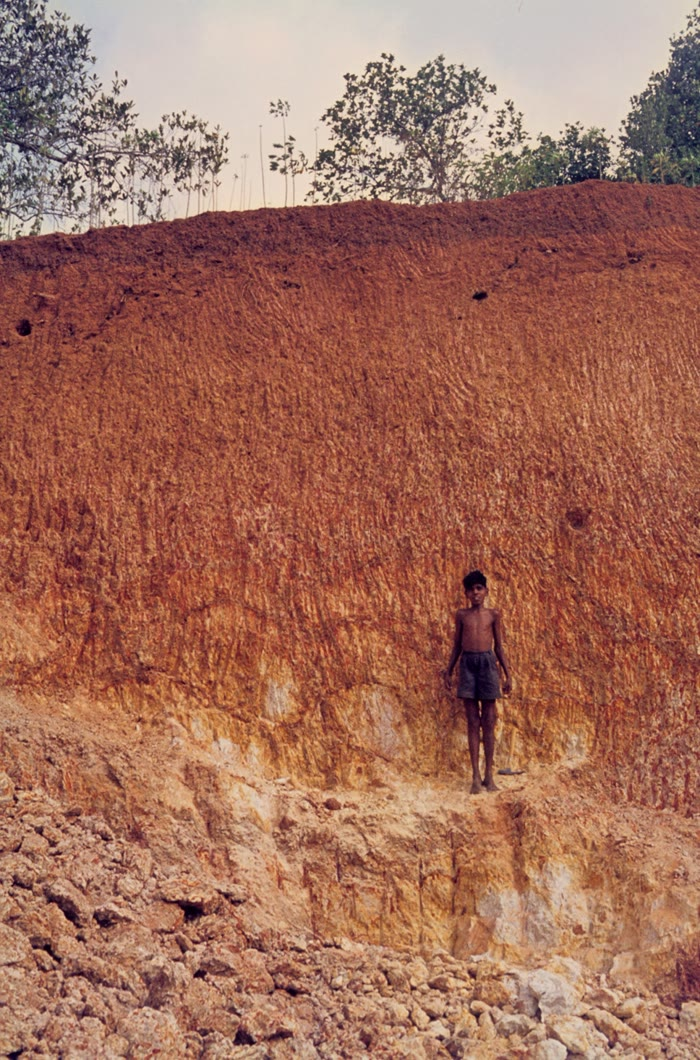
\includegraphics[height=8.5cm]{images/book2/g10-laterite-kerala.jpg}

{\small مقطع تجوية على نيس غرانيتي في كيرالا، جنوب الهند: في الأسفل، صخر متحلل
مبقّع؛ وفوقه \omterm{def:g10:soil-formation:laterite}{لاتريت} بني ضعيف التصلب تحت تربة رقيقة. والصبي يعطي المقياس. الصورة:
فيرنر شيلمان، 1969 (CC~BY-SA~2.5).}
\end{omfigure}

\begin{recall}
التجوية تفتت الصخور في مكانها؛ والتعرية تحمل القطع بعيدًا؛ والترسيب يضعها في مكان
آخر (الكتاب 1، الصف 5). والصخور مكونة من معادن، كالكوارتز والفلسبارات والميكا في
الغرانيت (الكتاب 1، الصف 6). والتربة طبقة حية من حبيبات معدنية ودبال وماء وهواء
وكائنات حية؛ وتحوّل المحللات المادة الميتة إلى دبال؛ وتوصف التربة بطبقاتها، أو
آفاقها (كتب الأحياء). وفي الأكسدة تفقد مادة إلكترونات، غالبًا باتحادها مع الأكسجين
(كتب الكيمياء).
\end{recall}

\section{من الصخر إلى التربة}

التجوية الفيزيائية --- تفلّق الصخر بالصقيع، والتسخين والتبريد، والجذور --- تفتت
الصخر قطعًا دون أن تغير معادنه. أما \omterm{def:g10:soil-formation:chemical-weathering}{التجوية الكيميائية} فتغير المعادن نفسها. وهما
معًا، على مدى أزمنة طويلة، يحوّلان أعلى الصخر الصلب إلى غطاء مفكك يزداد سماكة نحو
الأسفل كلما نخرت التجوية الصخر الذي تحته.

\begin{definition}[الصخر الأم؛ السابروليت]\label{def:g10:soil-formation:weathering-profile}
\emph{الصخر الأم}\index{صخر أم} للتربة هو الصخر الذي تكوّن منه جزؤها المعدني.
و\emph{السابروليت}\index{سابروليت} صخر تحلل في مكانه بالتجوية: لين وترابي، لكنه ما
زال يُظهر حبيبات الصخر الأم وبنيته. و\emph{مقطع التجوية} هو العمود كله من الصخر
السليم، عبر السابروليت، إلى التربة في الأعلى.
\end{definition}
% ledger: usgs:saprolite

قد يكون \omterm{def:g10:soil-formation:weathering-profile}{السابروليت} سميكًا. فتحت التلال المتموجة على امتداد الجانب الشرقي من جبال
الأبالاش، في شرق الولايات المتحدة، يبلغ نحو
\qty{46}{m} (150 قدمًا) في بعض الأماكن، وإن كانت سماكته تتفاوت كثيرًا من مكان إلى
آخر؛ والتربة ليست إلا جزأه العلوي.
% ledger: usgs:saprolite

\begin{omfigure}
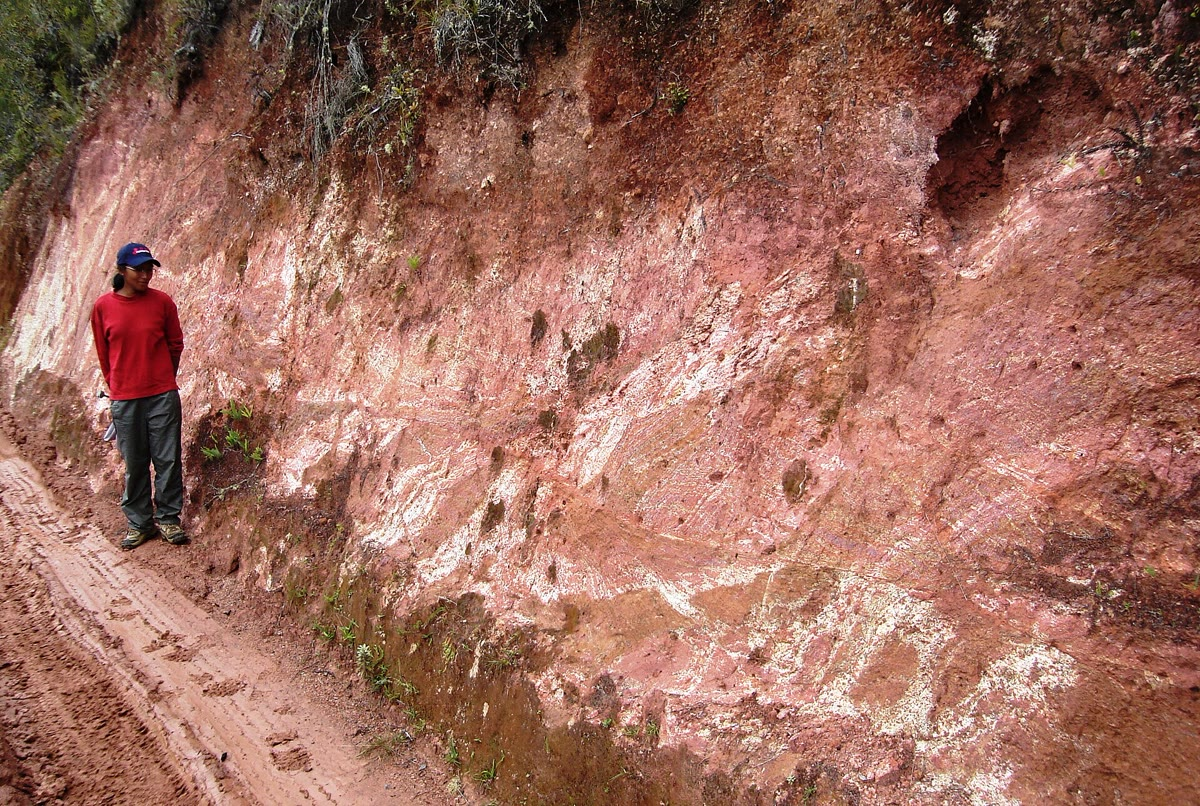
\includegraphics[width=0.8\linewidth]{images/book2/g10-saprolite-madagascar.jpg}

{\small \omterm{def:g10:soil-formation:weathering-profile}{سابروليت} في طريق مشقوق وسط مدغشقر: النيس القديم، المتحلل في مكانه، ما زال
يُظهر أشرطته خطوطًا من الطين الأبيض في التراب الأحمر. الصورة: ديوريت
(CC~BY-SA~3.0).}
\end{omfigure}

\begin{omfigure}
\begin{tikzpicture}[font=\footnotesize]
  % humid tropical column
  \begin{scope}
    \fill[omThm!45!brown!60] (0,5.4) rectangle (1.8,6.0);
    \fill[omThm!70!orange!70] (0,4.2) rectangle (1.8,5.4);
    \fill[omThm!25!orange!35] (0,1.2) rectangle (1.8,4.2);
    \foreach \y in {1.5,2.1,2.7,3.3,3.9} \draw[white!80!black, thick] (0.1,\y) -- (1.7,\y+0.15);
    \fill[black!30] (0,0) rectangle (1.8,1.2);
    \foreach \x/\y in {0.3/0.3,0.9/0.7,1.4/0.2,0.5/0.9,1.2/1.0} \draw[black!55] (\x,\y) -- ++(0.2,0.08);
    \draw[black!60] (0,0) rectangle (1.8,6.0);
    \node[anchor=north, align=center] at (0.9,-0.1) {المناطق المدارية\\الرطبة};
  \end{scope}
  % temperate column
  \begin{scope}[xshift=3.2cm]
    \fill[omThm!45!brown!60] (0,2.2) rectangle (1.8,2.6);
    \fill[omThm!25!orange!35] (0,1.2) rectangle (1.8,2.2);
    \foreach \y in {1.5,1.9} \draw[white!80!black, thick] (0.1,\y) -- (1.7,\y+0.15);
    \fill[black!30] (0,0) rectangle (1.8,1.2);
    \foreach \x/\y in {0.3/0.3,0.9/0.7,1.4/0.2,0.5/0.9,1.2/1.0} \draw[black!55] (\x,\y) -- ++(0.2,0.08);
    \draw[black!60] (0,0) rectangle (1.8,2.6);
    \node[anchor=north, align=center] at (0.9,-0.1) {مناخ\\معتدل};
  \end{scope}
  % labels
  \draw[black!50] (5.3,5.7) -- (2.0,5.7); \node[anchor=west] at (5.4,5.7) {التربة};
  \draw[black!50] (5.3,4.8) -- (2.0,4.8); \node[anchor=west, align=left] at (5.4,4.8) {اللاتريت: أحمر، غني بأكاسيد\\الحديد والألومنيوم};
  \draw[black!50] (5.3,3.4) -- (2.0,3.4); \node[anchor=west, align=left] at (5.4,3.4) {السابروليت: صخر متحلل\\في مكانه، محتفظ ببنيته};
  \draw[black!50] (5.3,0.6) -- (5.0,0.6); \node[anchor=west] at (5.4,0.6) {الصخر الأم السليم};
\end{tikzpicture}

{\small مقطعا تجوية على الصخر نفسه (رسم تخطيطي، بغير مقياس): تحت مناخ حار رطب
يكون المقطع أسمك بكثير وأعلاه \omterm{def:g10:soil-formation:laterite}{لاتريت}؛ وتحت مناخ معتدل يحمل \omterm{def:g10:soil-formation:weathering-profile}{سابروليت} أرق
التربة.}
\end{omfigure}

\section{التجوية الكيميائية}

\begin{definition}[التجوية الكيميائية]\label{def:g10:soil-formation:chemical-weathering}
\emph{التجوية الكيميائية}\index{تجوية كيميائية} هي تحوّل معادن الصخر بتفاعلات مع
الماء ومع الغازات التي يحملها، ثاني أكسيد الكربون والأكسجين: فبعض المعادن يذوب،
وبعضها الآخر يتحول إلى معادن جديدة، مستقرة عند سطح الأرض.
\end{definition}

يذيب ماء المطر قليلًا من ثاني أكسيد الكربون من الهواء، وأكثر بكثير وهو يتسرب عبر
التربة، حيث تزفره الجذور والمحللات. ويكوّن جزء من الغاز الذائب حمض الكربونيك، الذي
يحرر أيونات الهيدروجين:
\begin{center}
\ce{CO2 + H2O -> H+ + HCO3-}
\end{center}
وأيونات الهيدروجين هذه تهاجم المعادن.

\begin{definition}[الحلمهة]\label{def:g10:soil-formation:hydrolysis}
\emph{الحلمهة}\index{حلمهة} هي \omterm{def:g10:soil-formation:chemical-weathering}{التجوية الكيميائية} لمعدن سيليكاتي بالماء وأيونات
الهيدروجين فيه: تحل أيونات الهيدروجين محل أيونات الفلز في المعدن، فتذهب هذه في
المحلول، ويُعاد بناء بقية المعدن معدنًا طينيًا.
\end{definition}

\begin{proposition}[حلمهة الفلسبار]\label{prop:g10:soil-formation:hydrolysis}
يتحول فلسبار البوتاسيوم الأورثوكلاز، \ce{KAlSi3O8}، \omterm{def:g10:soil-formation:hydrolysis}{بالحلمهة}
إلى \omterm{def:g10:soil-formation:clay}{المعدن الطيني} الكاولينيت، \ce{Al2Si2O5(OH)4}؛ ويحمل الماء أيونات البوتاسيوم
والسيليكا الذائبة، \ce{H4SiO4}:
\begin{center}
\ce{2 KAlSi3O8 + 2 H+ + 9 H2O -> Al2Si2O5(OH)4 + 2 K+ + 4 H4SiO4}
\end{center}
\end{proposition}
% ledger: webmineral:formulas

\begin{proof}[تحقق]
عُدّ كل عنصر في الطرفين. البوتاسيوم: 2 و2. الألومنيوم: 2 و2.
السيليكون: 6 و$2 + 4 = 6$. الأكسجين: $16 + 9 = 25$ و$9 + 16 = 25$.
الهيدروجين: $2 + 18 = 20$ و$4 + 16 = 20$. الشحنة: $+2$ و$+2$.
\end{proof}

\begin{proposition}[ذوبان الكالسيت]\label{prop:g10:soil-formation:calcite}
يذوب الكالسيت، \ce{CaCO3}، معدن الحجر الجيري، ذوبانًا تامًا في الماء
الذي يحمل ثاني أكسيد الكربون؛ فلا يبقى شيء صلب:
\begin{center}
\ce{CaCO3 + CO2 + H2O -> Ca^2+ + 2 HCO3-}
\end{center}
\end{proposition}
% ledger: webmineral:formulas

يُهاجَم الحديد بطريقة ثالثة. ففي المعادن الداكنة للصخر، كالميكا السوداء في
الغرانيت، يكون الحديد في الصورة المختزلة \ce{Fe^2+}. فيؤكسده الأكسجين الذي يحمله
الماء، ويبقى الحديد(III) على شكل أكاسيد غير ذائبة: الغوثيت الأصفر البني، \ce{FeO(OH)}،
والهيماتيت الأحمر،
\ce{Fe2O3}. وللغوثيت:
\begin{center}
\ce{4 Fe^2+ + O2 + 6 H2O -> 4 FeO(OH) + 8 H+}
\end{center}
وهذه الأكاسيد تلوّن الصخور المتجوّية والترب بالأصفر والبني والأحمر.
% ledger: webmineral:formulas

لا تتجوّى المعادن كلها بالوتيرة نفسها. ففي غرانيت يتجوّى، تصدأ الميكا السوداء
وتتحول الفلسبارات إلى طين، أما حبيبات الكوارتز، شبه غير الذائبة، فتخرج دون تغير:
وتنتهي رملًا.

\begin{example}[تجوية الغرانيت]\label{ex:g10:soil-formation:granite}
% ledger: webmineral:formulas (masses computed in figdata/grade-10/soil_rates.py)
يحتوي كيلوغرام من الأورثوكلاز على $1000/278.33 \approx \qty{3.59}{mol}$ من
\ce{KAlSi3O8}. وبحسب المعادلة، يعطي مولان من الأورثوكلاز مولًا واحدًا من
الكاولينيت: $3.59/2 \approx \qty{1.80}{mol}$، أي $1.80 \times 258.16
\approx \qty{464}{g}$ من الطين. والبوتاسيوم، $14.05~\%$ من كتلة
الأورثوكلاز، أي \qty{140.5}{g}، و$2 \times 3.59 = \qty{7.19}{mol}$ من السيليكا
تذهب في المحلول. ومن غرانيت مكوّن من الكوارتز والفلسبارات والميكا، تترك التجوية
رملًا (الكوارتز)، وطينًا (من الفلسبارات والميكا) وأكاسيد حديد، وترسل البوتاسيوم
والصوديوم والكالسيوم والسيليكا إلى الأنهار.
\end{example}

\section{الطين والدبال}

\begin{definition}[المعدن الطيني]\label{def:g10:soil-formation:clay}
\emph{المعدن الطيني}\index{معدن طيني} سيليكات مبنية من صفائح رقيقة من الذرات
مكدسة بعضها فوق بعض، تتكون بالتجوية، وتوجد على شكل رقائق أصغر بكثير من حبيبات
الرمل. والكاولينيت أحدها.
\end{definition}
% ledger: webmineral:formulas

تحمل أسطح الرقائق الطينية شحنات كهربائية سالبة. فهي تمسك الأيونات الموجبة ---
البوتاسيوم \ce{K+}، والكالسيوم \ce{Ca^2+}، والمغنيسيوم
\ce{Mg^2+}، والأمونيوم \ce{NH4+} --- التي كان المطر سيجرفها لولا ذلك. والدبال يفعل
الشيء نفسه. ويكوّن الطين والدبال، مرتبطين معًا،
\emph{المعقد الطيني الدبالي}، مخزن التربة من المغذيات المعدنية: فالجذر يحرر أيونات
الهيدروجين ويأخذ في مقابلها البوتاسيوم أو الكالسيوم الممسوك على
الرقائق.

\begin{omfigure}
\begin{tikzpicture}[font=\footnotesize, >={Stealth[length=2mm]}]
  \foreach \y in {0,0.7,1.4} {
    \fill[omExo!35, draw=black!60] (0,\y) rectangle (7.2,\y+0.3);
    \foreach \x in {0.3,0.9,...,7.0} \node[font=\tiny, black!70] at (\x,\y+0.15) {$-$};
  }
  \foreach \x/\ion in {0.7/K^+, 1.9/Ca^{2+}, 3.1/K^+, 4.3/Mg^{2+}, 5.5/NH_4^+, 6.7/K^+} {
    \fill[omThm!20, draw=omThm!80!black] (\x,2.1) circle (0.4);
    \node[font=\scriptsize] at (\x,2.1) {$\mathrm{\ion}$};
  }
  \foreach \x in {1.3, 3.7, 6.1} \fill[omThm!20, draw=omThm!80!black] (\x,0.5) circle (0.17);
  \foreach \x in {2.5, 4.9} \fill[omThm!20, draw=omThm!80!black] (\x,1.2) circle (0.17);
  \node[anchor=north] at (3.6,-0.1) {صفائح طينية سالبة الشحنة، بينها أيونات موجبة};
  \node[anchor=south] at (3.1,2.5) {أيونات موجبة ممسوكة على الأسطح};
  % root and exchange
  \draw[line width=2.2pt, brown!60!black] (9.6,3.4) .. controls (9.3,2.6) and (8.9,2.2) .. (8.1,2.0);
  \node[anchor=east] at (9.25,3.3) {الجذر};
  \draw[->, omDef!80!black, thick] (8.0,2.2) .. controls (7.6,2.6) and (7.2,2.6) .. (6.95,2.3);
  \node[anchor=south, omDef!80!black] at (7.5,2.55) {\foreignlanguage{arabic}{يعطي \ce{H+}}};
  \draw[->, omThm!80!black, thick] (6.95,1.8) .. controls (7.3,1.5) and (7.7,1.6) .. (8.0,1.85);
  \node[anchor=north, omThm!80!black] at (7.8,1.55) {\foreignlanguage{arabic}{يأخذ \ce{K+}}};
\end{tikzpicture}

{\small المعقد الطيني الدبالي (رسم تخطيطي): صفائح طينية سالبة الشحنة تمسك
أيونات موجبة على أسطحها وبينها؛ والجذر يبادل أيونات الهيدروجين بهذه
المغذيات.}
\end{omfigure}

\section{الترب والمناخ}

تحتاج \omterm{def:g10:soil-formation:chemical-weathering}{التجوية الكيميائية} إلى الماء، وهي ككل التفاعلات تقريبًا تجري أسرع في الدفء.
فحيث يكون المناخ حارًا ورطبًا معًا، يتحلل الصخر إلى أعمق وأبعد حد: فتتحول الفلسبارات
كليًا إلى طين، بل يُحمل جزء كبير من السيليكا نفسها، ويكون ما يبقى غنيًا بأقل العناصر
ذوبانًا، الحديد والألومنيوم.

\begin{definition}[اللاتريت]\label{def:g10:soil-formation:laterite}
\emph{اللاتريت}\index{لاتريت} مادة شديدة التجوية من المناخات الحارة الرطبة، حمراء
أو بنية، مكوّنة أساسًا من أكاسيد الحديد والألومنيوم ومن الكاولينيت، أُزيل منها كل
ما يذوب تقريبًا.
\end{definition}

تحت المناخات الباردة، المتجمدة معظم السنة، وتحت المناخات الجافة، حيث الماء شحيح،
تكون \omterm{def:g10:soil-formation:chemical-weathering}{التجوية الكيميائية} بطيئة: فالترب رقيقة والصخر قريب تحتها. وبين القطبين وخط
الاستواء، يكون عمق التجوية أكبر ما يكون تحت الغابات المدارية الرطبة وأصغر ما يكون في
الصحارى والمناطق القطبية.

\begin{omfigure}
\begin{tikzpicture}[font=\footnotesize]
  \fill[black!25] (0,-0.2) -- (0,-0.5) .. controls (1.5,-0.6) and (2.5,-1.4) .. (3.4,-1.2)
     .. controls (4.2,-1.0) and (4.6,-0.55) .. (5.2,-0.5) .. controls (6.0,-0.5) and (6.6,-1.6) .. (7.6,-3.0)
     .. controls (8.2,-3.6) and (9.0,-3.6) .. (10,-3.4) -- (10,-3.8) -- (0,-3.8) -- cycle;
  \fill[omThm!25!orange!35] (0,0) -- (10,0) -- (10,-3.4) .. controls (9.0,-3.6) and (8.2,-3.6) .. (7.6,-3.0)
     .. controls (6.6,-1.6) and (6.0,-0.5) .. (5.2,-0.5) .. controls (4.6,-0.55) and (4.2,-1.0) .. (3.4,-1.2)
     .. controls (2.5,-1.4) and (1.5,-0.6) .. (0,-0.5) -- cycle;
  \draw[black!60] (0,0) -- (10,0);
  \node[anchor=south] at (0.6,0.05) {قطبي};
  \node[anchor=south] at (3.2,0.05) {معتدل};
  \node[anchor=south] at (5.3,0.05) {صحراوي};
  \node[anchor=south] at (6.8,0.05) {سافانا};
  \node[anchor=south] at (9.0,0.05) {غابة مدارية};
  \node[anchor=north] at (0.4,-3.85) {القطب};
  \node[anchor=north] at (9.6,-3.85) {خط الاستواء};
  \node[black!70] at (2.0,-2.6) {صخر سليم};
  \node[black!80] at (8.35,-1.0) {صخر متجوٍّ وتربة};
\end{tikzpicture}

{\small عمق التجوية من قطب إلى خط الاستواء (رسم تخطيطي، والأعماق بغير مقياس): رقيق
تحت المناخات القطبية والصحراوية، ومتوسط تحت المناخات المعتدلة، وأكبر ما يكون تحت
الغابات المدارية الرطبة.}
\end{omfigure}

\section{بطيئة التكوّن، سريعة الضياع}

ما سرعة تكوّن التربة؟ لقد قيس إنتاج التربة، أي المعدل الذي تحوّل به التجوية الصخر
إلى تربة عند قاعدة المقطع، في مواقع كثيرة حول العالم، وكذلك المعدل الذي تُعرّى به
التربة من السطح. ويعطي تجميعٌ لهذه القياسات المعدلات النموذجية (الوسيطة) الواردة
أدناه، معبَّرًا عن كل منها بسماكة من التربة في السنة.
% ledger: montgomery:rates

\begin{omfigure}
\begin{tikzpicture}
\begin{axis}[omrecord, width=0.82\linewidth, height=5.6cm, ymode=log, log origin=infty, ymin=0.005,
  ymax=5, ybar, bar width=16pt, xtick={0,1,2,3,4}, xmin=-0.6, xmax=4.6,
  xticklabels={{إنتاج\\التربة}, {التعرية تحت\\الغطاء النباتي الأصلي}, {التعرية\\الجيولوجية}, {الزراعة\\الحافظة}, {الحراثة\\التقليدية}},
  xticklabel style={align=center, font=\scriptsize},
  ylabel={\foreignlanguage{arabic}{المعدل بوحدة \babelsublr{\unit{mm}} في السنة}}, tick label style={font=\small}, label style={font=\small},
  nodes near coords, nodes near coords style={font=\scriptsize}, point meta=explicit symbolic]
\addplot[fill=omDef!45, draw=omDef!80!black] table[x=idx, y=rate_mm_yr, meta=rate_mm_yr] {figdata/out/grade-10-soil_rates-rates.dat};
\end{axis}
\end{tikzpicture}

{\small المعدلات الوسيطة لإنتاج التربة وتعريتها من تجميع عالمي للقياسات، بالمليمترات
من التربة في السنة (مقياس لوغاريتمي: كل خطوة عشرة أضعاف التي تحتها). البيانات:
مونتغمري (2007)،
\emph{وقائع الأكاديمية الوطنية للعلوم}.}
\end{omfigure}
% ledger: montgomery:rates

تحت الغطاء النباتي الطبيعي تُعرّى التربة بالسرعة التي تتكون بها تقريبًا، نحو
\qty{0.02}{mm} في السنة: أي سنتيمتر في نحو ستة قرون. وتحت الحراثة التقليدية، التي
تترك الأرض عارية بين المحاصيل، يبلغ المعدل الوسيط للتعرية
\qty{1.5}{mm} في السنة، أي تسعين ضعف معدل إنتاج التربة. وتحت الزراعة الحافظة، التي
تقلّب التربة أقل وتبقيها مغطاة، ينخفض الوسيط إلى \qty{0.08}{mm} في السنة، وهو أقرب
بكثير إلى معدل
الإنتاج.
% ledger: montgomery:rates (ratios computed in figdata/grade-10/soil_rates.py)

\begin{method}[مقارنة معدل تكوّن بمعدل تعرية]\label{met:g10:soil-formation:rates}
\begin{enumerate}
  \item عبّر عن المعدلين بالوحدة نفسها (المليمترات في السنة).
  \item الفقدان الصافي هو معدل التعرية $E$ مطروحًا منه معدل الإنتاج $P$.
  \item تُفقد تربة سماكتها $S$ في $T = S/(E - P)$ سنة؛ وإذا كان
        $E \le P$، فالتربة لا تُفقد.
  \item ويستغرق تكوين سماكة $S$ من لا شيء $S/P$ سنة.
\end{enumerate}
\end{method}
% ledger: montgomery:lifetime

بهذه المعدلات، يستغرق تكوّن متر من التربة نحو $1000/0.017 \approx 59\,000$
سنة، ويمكن أن يُفقد تحت الحراثة التقليدية في نحو
$1000/(1.537 - 0.017) \approx 660$ سنة. فعلى المقاييس الزمنية البشرية، التربة
مورد لا يتجدد.
% ledger: montgomery:rates, montgomery:lifetime

\begin{omfigure}
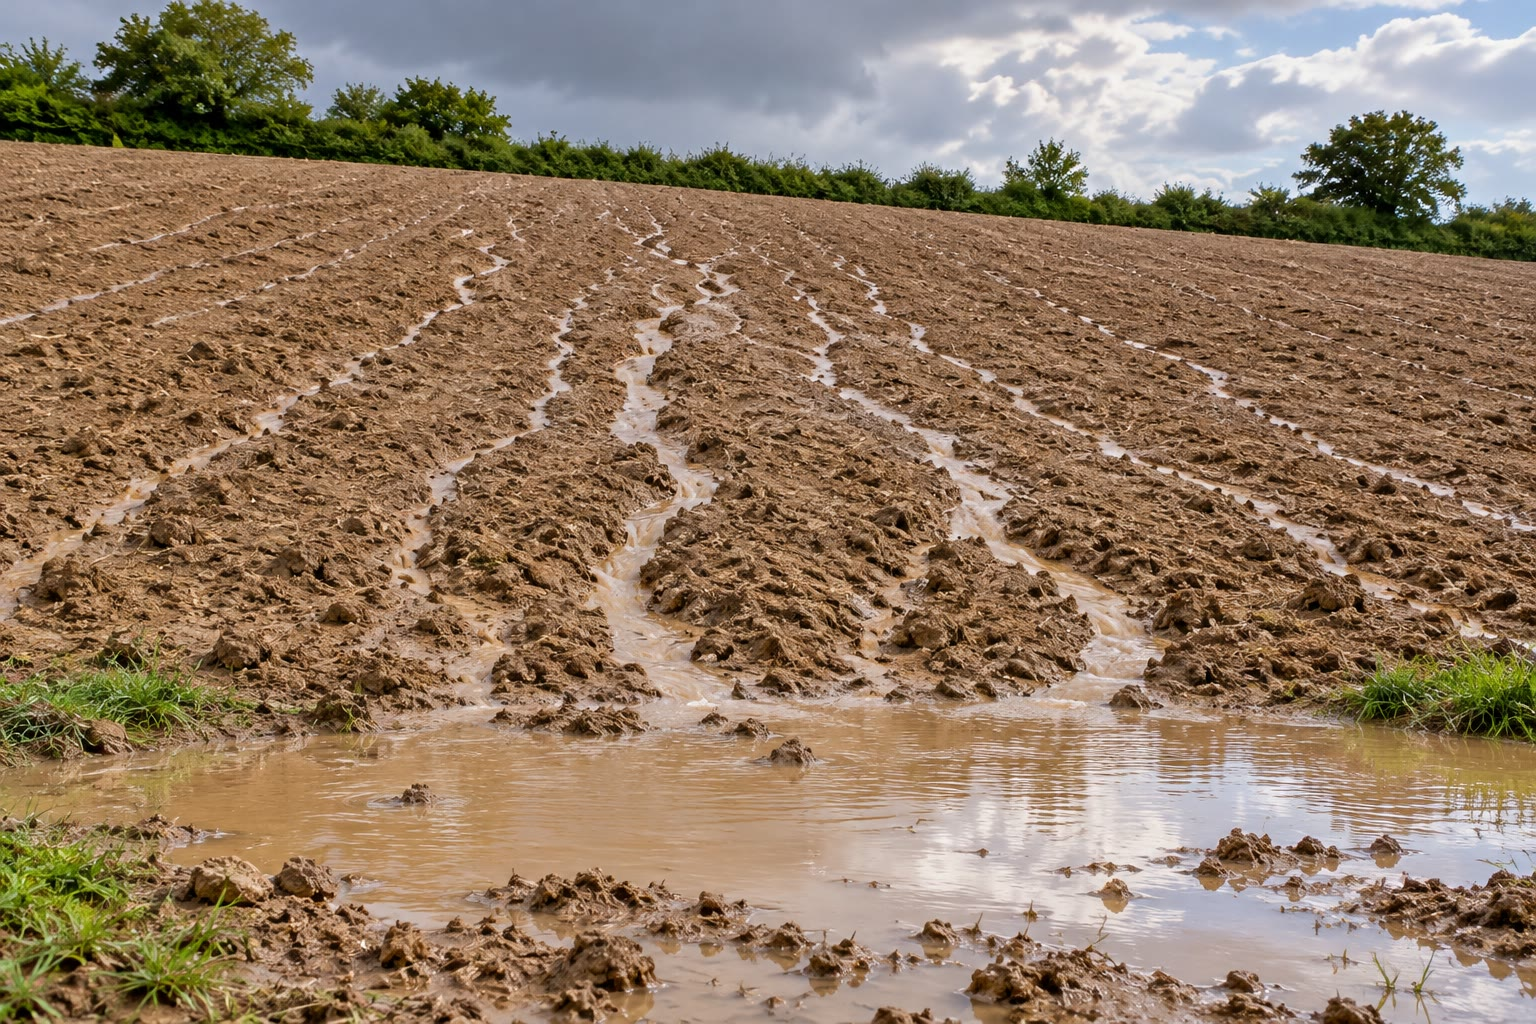
\includegraphics[width=0.72\linewidth]{images/book2/ai/g10-ploughed-rills.jpg}

{\small حقل محروث بعد عاصفة شديدة: حفر الجريان السطحي قنوات صغيرة، أو مسيلات، نزولًا
على المنحدر وحمل التربة إلى بركة موحلة عند
أسفله.}
\end{omfigure}

\section{تمارين}

\begin{exercise}[$\star$]\label{exo:g10:soil-formation:1}
عرّف \omterm{def:g10:soil-formation:chemical-weathering}{التجوية الكيميائية} \omterm{def:g10:soil-formation:hydrolysis}{والحلمهة}.
\end{exercise}

\begin{exercise}[$\star$]\label{exo:g10:soil-formation:2}
ما \omterm{def:g10:soil-formation:weathering-profile}{السابروليت}؟ وكيف تميّز \omterm{def:g10:soil-formation:weathering-profile}{السابروليت} من تربة تكوّنت في رمل جلبه
نهر؟
\end{exercise}

\begin{exercise}[$\star$]\label{exo:g10:soil-formation:3}
سمِّ نواتج تجوية الغرانيت: إلامَ يتحول كل واحد من معادنه الرئيسية
الثلاثة؟
\end{exercise}

\begin{exercise}[$\star$]\label{exo:g10:soil-formation:4}
لماذا تكون الصخور المتجوّية والترب المدارية في الغالب حمراء أو صفراء أو بنية؟
\end{exercise}

\begin{exercise}[$\star$]\label{exo:g10:soil-formation:5}
باستعمال المخطط العمودي، أعطِ المعدل الوسيط لإنتاج التربة والمعدل الوسيط
للتعرية تحت الحراثة التقليدية. وكم مرة يفوق الثاني
الأول؟
\end{exercise}

\begin{exercise}[$\star\star$]\label{exo:g10:soil-formation:6}
تحقق من أن معادلة ذوبان الكالسيت موزونة، لكل عنصر
وللشحنة.
\end{exercise}

\begin{exercise}[$\star\star$]\label{exo:g10:soil-formation:7}
يذوب الحجر الجيري ذوبانًا تامًا، أما الغرانيت فيترك رملًا وطينًا. فسّر الفرق
باستعمال تفاعلَي الفصل.
\end{exercise}

\begin{exercise}[$\star\star$]\label{exo:g10:soil-formation:8}
فسّر كيف يحتفظ المعقد الطيني الدبالي بالبوتاسيوم في تربة يغسلها المطر، وكيف يأخذه
الجذر.
\end{exercise}

\begin{exercise}[$\star\star$]\label{exo:g10:soil-formation:9}
أعطِ سببين لتكوّن \omterm{def:g10:soil-formation:laterite}{اللاتريت} تحت المناخات الحارة الرطبة لا تحت الباردة
أو الجافة.
\end{exercise}

\begin{exercise}[$\star\star$]\label{exo:g10:soil-formation:10}
المعدل الوسيط لإنتاج التربة \qty{0.017}{mm} في السنة. كم يستغرق تكوين
\qty{1}{cm} و\qty{30}{cm} و\qty{1}{m} من التربة؟
\end{exercise}

\begin{exercise}[$\star\star$]\label{exo:g10:soil-formation:11}
كثيرًا ما تُعطى معدلات التعرية كتلةً من التربة لكل هكتار في السنة. فبكثافة تربة
قدرها \qty{1200}{kg/m^3}، ما الكتلة التي يمثلها فقدان
\qty{1.5}{mm} في السنة على هكتار واحد (\qty{10000}{m^2})؟
\end{exercise}

\begin{exercise}[$\star\star\star$]\label{exo:g10:soil-formation:12}
تكوّن \omterm{def:g10:soil-formation:weathering-profile}{سابروليت} سماكته \qty{46}{m} تحت تلال منطقة معتدلة. فلو تقدمت التجوية
داخل الصخر بمعدل \qty{0.017}{mm} في السنة، فكم كان سيستغرق ذلك؟ وماذا توحي
الإجابة عن عمر مثل هذا
المشهد الطبيعي؟
\end{exercise}

\begin{exercise}[$\star\star\star$]\label{exo:g10:soil-formation:13}
اكتب معادلة أكسدة \ce{Fe^2+} إلى الغوثيت الواردة في
الفصل وتحقق منها. ثم اكتب معادلة أكسدة \ce{Fe^2+} إلى
الهيماتيت، \ce{Fe2O3}، بالأكسجين والماء مع تحرر \ce{H+}، ووازنها.
\end{exercise}

\begin{exercise}[$\star\star\star$]\label{exo:g10:soil-formation:14}
تحت الزراعة الحافظة يبلغ المعدل الوسيط للتعرية \qty{0.082}{mm} في
السنة. فمع إنتاج للتربة قدره \qty{0.017}{mm} في السنة، كم يستغرق
فقدان \qty{30}{cm} من التربة؟ قارن بالحراثة التقليدية.
\end{exercise}

\begin{exercise}[$\star\star\star$]\label{exo:g10:soil-formation:15}
غرانيت يحتوي على \qty{30}{\percent} أورثوكلاز كتلةً. ما كتلة
الكاولينيت التي تتكون حين يتجوّى كل الأورثوكلاز في طن واحد من هذا الغرانيت، وما كتلة
البوتاسيوم المتحررة؟
\end{exercise}

\section{مسألة: عمر التربة}

\begin{problem}[{مسألة نهاية الأسبوع --- من الصخر إلى الحقل ثم إلى النهر}]
% ledger: montgomery:rates, montgomery:lifetime, webmineral:formulas (values computed in figdata/grade-10/soil_rates.py)

\begin{center}
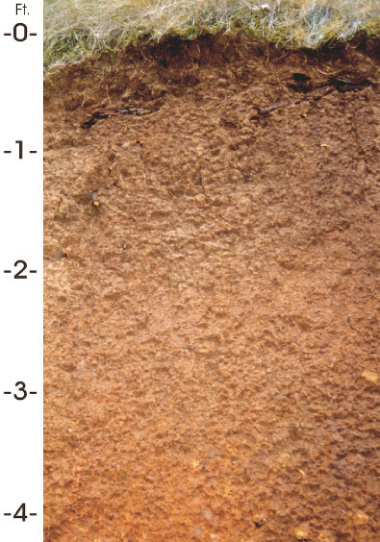
\includegraphics[height=6cm]{images/book2/g10-nrcs-jory-soil.jpg}

{\small مقطع تربة، وعلى يساره مقياس بالأقدام (\num{1}~قدم =
\qty{0.3048}{m}). الصورة: دائرة حماية الموارد الطبيعية التابعة لوزارة الزراعة
الأمريكية (ملك عام).}
\end{center}
% the label sits after the photograph: at this page break tcolorbox discards a
% zero-height first part, and a label written in it is lost (undefined ref)
\label{pb:g10:soil-formation:1}

\medskip
\noindent\textbf{الجزء الأول --- مقطع.}
\begin{enumerate}
  \item يبلغ المقياس 4 أقدام قرب أسفل الصورة. فكم يساوي هذا العمق
        بالأمتار؟
  \item تبلغ الطبقة الداكنة في الأعلى نحو نصف قدم. فكم سماكتها،
        بالسنتيمترات؟
  \item ما الذي يعطي هذه الطبقة العليا لونها الداكن؟
  \item في الأسفل، التربة بنية مائلة إلى الحمرة. أي المعادن يعطيها هذا
        اللون، وكيف تكوّنت؟
  \item هل \omterm{def:g10:soil-formation:weathering-profile}{الصخر الأم} ظاهر في الصورة؟ وماذا تتوقع أن تجد
        تحت أسفل الصورة؟
\end{enumerate}

\medskip
\noindent\textbf{الجزء الثاني --- كيمياء غرانيت يتجوّى.}
\begin{enumerate}[resume]
  \item اكتب معادلة \omterm{def:g10:soil-formation:hydrolysis}{حلمهة} الأورثوكلاز.
  \item كم مولًا من الأورثوكلاز في \qty{1}{kg}
        (\qty{278.33}{g/mol})؟
  \item ما كتلة الكاولينيت (\qty{258.16}{g/mol}) التي تعطيها؟
  \item ما الذي يذهب مع الماء، وإلى أين يذهب؟
  \item ماذا يحدث لكوارتز الغرانيت؟
\end{enumerate}

\medskip
\noindent\textbf{الجزء الثالث --- التكوّن مقابل التعرية.}
\begin{enumerate}[resume]
  \item تتكون التربة بمعدل \qty{0.017}{mm} في السنة. كم يستغرق تكوين
        مقطع الجزء الأول؟
  \item تحت الحراثة التقليدية تُعرّى التربة بمعدل \qty{1.537}{mm} في
        السنة. ما الفقدان الصافي كل سنة؟
  \item كم كان مقطع الجزء الأول سيدوم؟
  \item قارن الزمنين في السؤالين 11 و13.
  \item تحت الغطاء النباتي الطبيعي، تبلغ التعرية \qty{0.013}{mm} في السنة. فهل
        تُفقد التربة؟
\end{enumerate}

\medskip
\noindent\textbf{الجزء الرابع --- عمر التربة.}
\begin{enumerate}[resume]
  \item اكتب الزمن $T$ اللازم لفقدان سماكة $S$ من التربة بدلالة
        $S$، ومعدل التعرية $E$، ومعدل الإنتاج $P$.
  \item احسب $T$ من أجل $S = \qty{30}{cm}$ تحت الحراثة التقليدية.
  \item احسب $T$ من أجل $S = \qty{30}{cm}$ تحت الزراعة الحافظة
        (\qty{0.082}{mm} في السنة).
  \item لماذا يمكن أن توصف التربة بأنها مورد لا يتجدد على المقاييس الزمنية
        البشرية؟
  \item كم يستغرق فقدان متر من التربة تحت الحراثة
        التقليدية؟
\end{enumerate}
\end{problem}
